\documentclass[11pt]{article}

\usepackage[margin=.8in,letterpaper]{geometry}
\usepackage{amsmath,bm}
\usepackage{txfonts} % must be loaded after amsmath?
\usepackage{siunitx}
\usepackage{enumitem}
\usepackage{graphicx}
\usepackage{tikz}
\usepackage{wrapfig}
\usepackage{authblk}
\usepackage{xcolor,colortbl}

\setlength{\parindent}{0pt}
\setlength{\parskip}{8pt}


\usetikzlibrary{decorations.pathmorphing,patterns}

\sisetup{
  detect-all,
  per-mode=symbol
}

\title{Topic 22: Wave Particle Duality\\Advanced Placement Physics}
\author{Timothy M.\ Leung\thanks{Ph.D. (Toronto), M.A.Sc. (Toronto), B.A.Sc.
    (British Columbia), \texttt{tleung@olympiadsmail.ca}}}
\affil{Olympiads School\\Toronto, Ontario, Canada}
\date{\today}

\newcommand{\pic}[2]{\includegraphics[width=#1\textwidth]{#2}}
\newcommand{\mb}[1]{\ensuremath\mathbf{#1}}

\begin{document}

\vspace{-2.5in}\maketitle



\begin{center}
  \begin{minipage}{.8\linewidth}
    \emph{Anyone who is not shocked by the quantum theory has not understood
      it.}
  
    \flushright{- Niels Bohr}
  \end{minipage}
\end{center}
The final topic in the AP Physics course at Olympiads School concerns one of
the most significant advancements in physics at the turn of the twentieth
century: the developement of the quantum theory. Unlike the development of the
theory of relativity (both special and general), which owes much to the
singular work by Albert Einstein, quantum mechanics was developed by many
leading scientists at the time. The material covered in this course deals
particularly the early development of the quantum theory, called
\textbf{wave mechanics}.

Earlier in this course, the difference between \emph{particles} and \emph{waves}
were discussed. However, 


\section{Quantization of Energy}

\subsection{Blackbody Radiation}

\begin{wrapfigure}{r}{.3\textwidth}%[ht]
  \centering
  \pic{.3}{800px-Black_body_realization.png}
  %\pic{.2}{../Black-body_realization.png}
  \caption{A blackbody}
  \label{fig:blackbody}
\end{wrapfigure}
The \textbf{blackbody} is a concept was coined by Gustav Kirchhoff in 1860. It
is an idealized object that absorbs all incident EM radiation, regardless of
frequency or angle of incidence. It is often modeled as a box (a ``cavity'')
with a mirror inside, and a hole where light (EM radiation) is allowed in, as
shown in Fig.\ref{fig:blackbody}. Some of the light reflects inside the cavity,
and some gets absorbed by the blackbody itself. Eventually, all the light
inside the cavity is absorbed.

A blackbody is in thermodynamic equilibrium; all of the absorbed energy is then
immediately radiated back as EM radiation, and the spectral distribution
depends only on temperature. A blackbody at room temperature appears black, as
most of the radiative energy is infrared and cannot be perceived by the human
eye. Although blackbodies do not exist in the universe, thermal radiation
spontaneously emitted by many ordinary objects can be approximated as blackbody
radiation.



\subsection{Rayleigh-Jeans Law and the Ultraviolet Catastrophe}

\begin{wrapfigure}{r}{.5\textwidth}
  \centering
  \pic{.5}{../1280px-Black_body.png}
\end{wrapfigure}
We can see that the peak of the emission spectrum shifts towards shorter
wavelengths as temperature increases.
\textbf{Wien's displacement law}\footnote{The law is obtained by
  considering the adiabatic expansion of the cavity in thermodynamic
  equilibrium} states that the spectral radiance of blackbody radiation peaks
at the wavelength $\lambda_{\text{peak}}$, given by:
\begin{equation}
  \lambda _{\text{peak}}=\frac {b}{T}
\end{equation}
where $T$ is the thermodynamic (absolute) temperature in, and $b$ is called
Wien's displacement constant, with a value of \SI{2.898e-3}{\metre\kelvin}.

Based on classical thermodynamics the power emitted by a blackbody should be
given by the \textbf{Rayleigh-Jean law}:
\begin{equation}
  P(\lambda,T)=8\pi kT\lambda^{-4}
\end{equation}
where $k$ is Boltzman's constant. This equation agrees with experimental
results for long wavelengths, but strongly disagrees for short wavelengths. As
$\lambda\rightarrow 0$, $P\rightarrow\infty$. This is known as the
\textbf{``ultra-violet catastrophe''}.

\subsection{Energy Quanta}

\begin{wrapfigure}{r}{.2\textwidth}
  \centering
  \pic{.2}{../20973-050-F6EEBFF1.jpg}
  Max Planck
\end{wrapfigure}
%    \column{.8\textwidth}
%    \begin{itemize}
Planck first made a strange modification in the classical calculations, and
derived a function of $P(\lambda,T)$ that agreed with experimental data for all
wavelengths. 
%    \item First found an empirical function to fit the data
Then he searched for a way to modify the usual calculations.
%    \end{itemize}

Planck postulated that the walls of a blackbody are composed of subatomic
electric oscillators\footnote{Think of oscillators as particles that are in
  harmonic motion, e.g.\ mass on a spring, or a pendulum}, which he called
``resonators''), whose exact nature were unknown to Planck. In this case, a
blackbody has billions of resonators vibrating at different frequencies, and
therefore emitting radiation at those frequencies.\footnote{Remember that for a
  wave, the frequency of disturbance at the source determines the frequency of
  the wave.} In classical physics, the resonators can have any value of energy,
and change its amplitude continuously. Howeve, in order to agree with
experimental results for the blackbody, Planck had to assume that energy
emitted the resonator must be \emph{discrete}. That is, when energy is emitted
from the resonator, it drops to the next lower energy level.

The total energy $E$ of \emph{any} harmonic oscillator can only be integral
multiples of $hf$:
\begin{equation}
  \boxed{E_{\textrm{res}}=nhf}
  \label{eq:nhf}
\end{equation}
%    \begin{center}
%      \begin{tabular}{l|c|c}
%        \rowcolor{pink}
%        \textbf{Quantity} & \textbf{Symbol} & \textbf{SI Unit} \\ \hline
%        Energy of the resonator & $E_{\textrm{res}}$ & \si{\joule}\\
where $n$ is the enegy level of the oscillator, $f$ is its frequency, and $h$
is a constant that we now call \textbf{Planck's constant}, which is
experimentally determined to be $h=\SI{6.626e-34}{\joule\second}$. This is
shown graphically in Fig.~\ref{fig:quantization}.
\begin{figure}[ht]
  \centering
  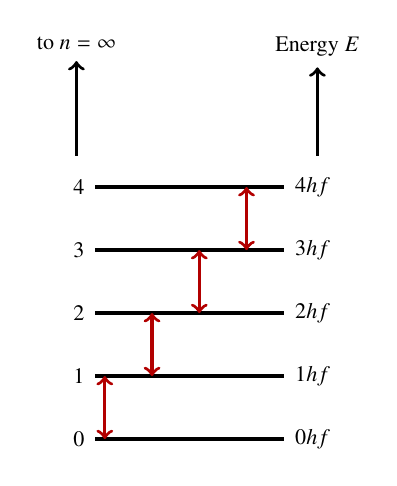
\begin{tikzpicture}[xscale=.6,yscale=.8]
    \foreach \y in {0,1,...,4} {
      \draw[very thick](0,\y)--(4,\y)
      node[pos=0,left] {\footnotesize $\y$}
      node[pos=1,right]{\footnotesize $\y hf$};
    }
    \foreach \y in {0,1,...,3} {
      \draw[very thick,red!70!black,<->](\y+.2,\y)--(\y+.2,\y+1);
    }
    \draw[very thick,->](4.7,4.5)--(4.7,5.9)
    node[pos=1,above]{\footnotesize Energy $E$};
    \draw[very thick,->](-.4,4.5)--(-.4,6)
    node[pos=1,above]{\footnotesize to $n=\infty$};
  \end{tikzpicture}
  \caption{Energy levels of a harmonic oscillator}
  \label{fig:quantization}
\end{figure}

As for his formula, it's called \textbf{Planck's law}:
\begin{equation}
  \boxed{
    P(\lambda,T)=\frac{2hc^2}{\lambda^5}\frac{1}{e^{\frac{hc}{\lambda k_BT}}-1}
  }
\end{equation}

\subsection{Classical vs. Quantum Oscillator}
This ``quantum'' behavior exists even for the simple pendulum that we studied
in mechanics topics in harmonic motion and circular motion.
\begin{figure}[ht]
  \centering
  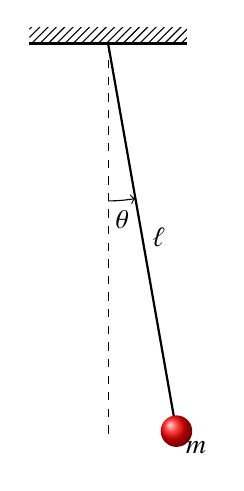
\begin{tikzpicture}
    \fill[pattern=north east lines] (-1,0) rectangle (1,0.2);
    \draw[very thick](-1,0)--(1,0);
    \begin{scope}[rotate=10]
      \draw[thick](0,0)--(0,-5) node[midway,right]{$\ell$};
      \tikzstyle{balloon}=[ball color=red];    
      \shade[balloon] (0,-5) circle (0.2) node[below right]{$m$};
    \end{scope}
    \draw[dashed,thin](0,0)--(0,-5);
    \draw[->](0,-2) arc(270:280:2) node[pos=0.5,below]{$\theta$};
  \end{tikzpicture}
\end{figure}
The natural frequency for an undamped pendulum with $\ell=\SI{1}{\metre}$ is
\begin{equation*}
  f=\frac{1}{2\pi}\sqrt{\frac{g}{\ell}}\approx\SI{.50}{\hertz}
\end{equation*}
According to Eq.~\ref{eq:nhf}, each energy level corresponds to 
\begin{displaymath}
  \Delta E=hf\approx\SI{3.3e-34}{\joule}
\end{displaymath}
For a pendulum with $m=$\SI{100}{\gram} and a maximum deflection of
$\theta=$\ang{10}, the total energy can be calculated at the maximum deflection,
when it consists entirely of gravitational potential energy:
\begin{displaymath}
  \frac{\Delta E}{E}=\frac{\Delta E}{mg\ell(1-\cos\theta)}
  \approx\num{2.2e-32}
\end{displaymath}
No wonder we can't observe it in a marcoscopic level!


\section{Waves as Particles}

Recall Maxwell's equation from earlier in the course:
\begin{align*}
  \nabla\cdot\mb{E} &= 0\\
  \nabla\cdot\mb{B} &= 0\\
  \nabla\times\mb{E} &=-\frac{\partial\mb{B}}{\partial t}\\
  \nabla\times\mb{B} &=\mu_o\varepsilon_o\frac{\partial\mb{E}}{\partial t}
\end{align*}
Solving the equations shows that disturbances in electric field $\mb{E}$ and
magnetic field $\mb{B}$ travel as an EM wave with a definite speed of
\begin{equation}
  c_0=\frac{1}{\sqrt{\varepsilon_0\mu_0}}=\SI{299792458}{\metre\per\second}
\end{equation}
in a vacuum. At that time, the speed of light was measured to be within one
percent of this value.\footnote{French physicist L\'{e}on Foucault measured the
  speed of light to be $\num{298000}\pm\SI{500}{\kilo\metre\per\second}$ using
  a rotating mirror experiment in 1862, around the time when Maxwell published
  his work. That measurement is within \SI{.60}{\percent} of the correct value.}
To prove that light is an EM wave, German physicist Heinrich Hertz
devised a ``spark gap experiment'' to generate frequencies in the range of
\SI{e14}{\hertz}.\footnote{The wavelenghts of light has been known as early as
  1801, after Thomas Young's double-slit experiments to show the wave
  interference behavior in light. Calculating the expected frequency of light
  only requires using the equation $v=f\lambda$ and then solving for $f$ using
  $v=c_0$.}
%  \begin{center}
%    \pic{.55}{Hertz_exp_2.png}
%  \end{center}
%  \begin{itemize}
%  \item\vspace{-.1in}Also showed that light has the same wavelengths as
%    predicted by Maxwell's equations
%  \item Discovered \textbf{photoelectric effect} that was caused by ultraviolet
%    radiation
%  \item Physicist who repeated his experiments did not have an explanation
%  \end{itemize}

\subsection{Photoelectric Effect}

At the end of Hertz's experimental results, he left a terse remark:
\begin{center}
  \begin{minipage}{.8\textwidth}
    \emph{``It is essential that the pole surfaces of the spark gap should be
      frequently repolished to ensure reliable operation of the spark.}
  \end{minipage}
\end{center}
This is now known as the \textbf{photoelectric effect} that was caused by
ultra-violet radiation. Hertz and other physicists who repeated his experiments
did not have a good explanation.

When EM waves (e.g. light) strike certain metals, electrons are knocked off the
surface, shown graphically in Fig.~\ref{fig:photo1}.
\begin{figure}[ht]
  \centering
  \pic{.9}{../73bacc9f2bf571752483a89ef6c61a94f07470f7.png}
  \caption{Photoelectric effect}
  \label{fig:photo1}
\end{figure}
When observing this \textbf{photoelectric effect}, physicists discovered that:
\begin{itemize}[noitemsep,topsep=0pt]
\item Increasing intensity of light knocked off more electrons, but doesn't
  change the maximum kinetic energy of the electrons, but
\item Changing the frequency of the light did change $K$ though, although
\item Below a certain frequency, \emph{no} electrons were emitted
\end{itemize}

\begin{wrapfigure}{r}{.2\textwidth}
  \centering
  \pic{.2}{../../21-Relativity/graphics/Einstein_patentoffice.png}
  Albert Einstein in 1905
\end{wrapfigure}
In his 1905 paper \emph{On a Heuristic Viewpoint Concerning the Production and
  Transformation of Light}, Einstein postulated that light is not continuous
wave, but a collection of discrete energy packets (photons), each with energy
$E=hf$, in agreement with Planck (Eq.~\ref{eq:nhf}). In this case, the
maximum kinetic energy $K_\mathrm{max}$ of a ``photoelectron'' is a simple
equation:
\begin{equation}
  \boxed{K_\mathrm{max}=
    \begin{cases}
      hf-\varphi & \text{if }hf>\varphi\\
      0          & \text{otherwise}
    \end{cases}
  }
  \label{eq:photoelectric1}
\end{equation}
where $f$ is frequency of the the incident EM radiation, $h$ is Planck's
constant, and $\varphi$ (measured in \si{\joule} or more commonly, in
\si{\electronvolt}) is the \textbf{work function} that is specific to the
metal.\footnote{Although $\varphi$ is called the work \emph{function}, it is
  merely an experimentally-determined constant for a particular metal.}
%    \end{tabular}
%  \end{center}
%  Einstein may have been alerted to the fact that the blackbody radiation curve
%  resembles the distribution of energies in a gas
It is the minimum energy required to remove an electron from a solid to a point
immediately outside the solid surface. The minimum frequency at which electrons
will be ejected is called the \textbf{threshold frequency} $f_0$. At this
frequency, $K=0$, and we can solve for $f_0$
\begin{equation}
  f_0=\frac{\varphi}{h}
\end{equation}
The slope the graph in Eq.~\ref{eq:photoelectric1} is always $h$, indepedent of
the metal. The work functions of common metals are shown in
Table~\ref{tabl:varphi}.
\begin{table}[ht]
  \centering
  \begin{tabular}{|c|c|}
    \rowcolor{pink}
    \hline
    \textbf{Metal} & $\varphi$ (\si{\electronvolt}) \\
    \hline
    Aluminum  & 4.28 \\ \hline
    Calcium   & 2.87 \\ \hline
    Cesium    & 2.14 \\ \hline
    Copper    & 4.65 \\ \hline
    Iron      & 4.50 \\ \hline
    Lead      & 4.25 \\ \hline
    Lithium   & 2.90 \\ \hline
    Nickel    & 5.15 \\ \hline
    Platinum  & 5.65 \\ \hline
    Potassium & 2.30 \\ \hline
    Tin       & 4.42 \\ \hline
    Tingsten  & 4.55 \\ \hline
    Zinc      & 4.33 \\ \hline
  \end{tabular}
  \caption{Work functions of common materials}
  \label{tabl:varphi}
\end{table}

Fig.~\ref{fig:zinc} shows the kinetic energy of the photoelectrons for zinc.
The threshold frequency occurs at $f_0=\SI{10.4e14}{\hertz}$, which is in the
ultra-violet range. The $y$-intercept of the graph is (not surprisingly)
$-\varphi=\SI{-4.33}{\electronvolt}$.
\begin{figure}[ht]
  \centering
  \pic{.4}{../550px-Photoelectric_effect_diagram.png}\\
  \textbf{THIS FIGURE MUST BE REPLACED BY MY OWN}
  \caption{Photoelectric equation for zinc}
  \label{fig:zinc}
\end{figure}



\subsection{Compton Scattering}

\begin{wrapfigure}{r}{.2\textwidth}
  \centering
  \pic{.2}{Arthur_Compton_1927.jpg}
  Arthur Holly Compton
\end{wrapfigure}
American physicist Arthur Holly Compton\footnote{1892--1962; Nobel Prize
  winner in 1927} studied x-ray scattering by free electrons.
\textbf{MORE INFORMATION REQUIRED FOR COMPTON SCATTERING}.

%  \begin{itemize}
%  \item Classical theory cannot account for the scattering behaviour
%  \item Frequency shift only depends on scattering angle
%  \item Prediction possible if treating the x-ray as photons with
%    momentum, just like a particle.
Using Einstein invariant\footnote{The Einstein invariant is defined as
  $E^2=p^2c^2+m^2c^4$. For massless particles, it simplifies to $E=pc$.} and
applied to a massless particle, the momentum carried by light can be expressed
as:
\begin{equation}
  \boxed{p=\frac{E}{c}=\frac{hf}{c}=\frac{h}{\lambda}}
  \label{eq:momentum-wavelength}
\end{equation}
This is a very odd expression, which treats photon both as a particle (with
momentum) and a wave (with a wavelength $\lambda$).
\begin{figure}[ht]
  \centering
  \pic{.5}{../compton2.png}\\
  \textbf{THIS FIGURE MUST BE REPLACED WITH MY OWN}
  \caption{Compton scattering}
  \label{fig:compton-scattering}
\end{figure}
If x-ray is treated as a photon (a particle!) with momentum $p=h/\lambda$ then
the interaction with the electron is merely an elastic collision, where both
momentum and energy are conserved after the collision i.e.
%In the collision between
%the x-ray photon and the electron, momentum is conserved
\begin{equation}
  \mb{p}=\mb{p}_e+\mb{p}'
\end{equation}
where $\mb{p}$ and $\mb{p}'$ are the momenta of the x-ray photon before and
after the interaction, and $\mb{p}_e$ is the momentum of the recoil electron
after the interaction. We can relate the magnitude of the momentum vectors by
the angle of the scattered photon:\footnote{This is literally using the cosine
  law to solve the vector problem.}
\begin{equation}
  p^2=p'^2+p_e^2 -2p'p_e\cos\theta
\end{equation}
Unfortunately, in this case, while the momentum of the photon is known, the
momentum of the recoil electron is not, so an extra equation is needed:
conservation of energy.


%  use Newton's laws of motion to predict both the recoil electron and scattered
%  x-ray!
%
%
%
%  \frametitle{Momentum of a Photon}
%  The momentum of a photon is proportional to Planck's constant and 
%  inversely proportional to its wavelength.
%
%\begin{equation}
%  \boxed{p=\frac{h}{\lambda}}
%\end{equation}
%  \begin{center}
%    \begin{tabular}{l|c|c}
%      \rowcolor{pink}
%      \textbf{Quantity} & \textbf{Symbol} & \textbf{SI Unit} \\ \hline
%      Momentum          & $p$ & \si{\kilo\gram.\metre/\second}\\
%      Planck's constant & $h$ & \si{\joule.\second}\\
%      Wavelength        & $\lambda$ & \si{\metre}
%    \end{tabular}
%  \end{center}
%
%
%%
%%  \frametitle{Example Problem}
%%  \textbf{Example 1}: Calculate the momentum of a photon of light that has
%%  frequency of $5.09\e{14}\mathrm{Hz}$.
%%
%

\section{Particles as Waves}

\begin{wrapfigure}{r}{.2\textwidth}
  \centering
  \pic{.2}{76562-004-66881FD5.jpg}
  Louis De Broglie
\end{wrapfigure}
If electromagnetic waves are really particles of energy, then are particles
(e.g.\ electrons) a wave of some sort? Louis De
Broglie\footnote{1892--1987; Nobel Prize winner in 1929}, while completing his
PhD in 1924, proposed a hypothesis: a particle can also have a wavelength.
%  \item Confirmed accidentally by the Davisson-Germer Experiment in 1927 (beam
%    of electron scattering on nickel crystal surface)
%  \end{itemize}
%
%  \vspace{.1in}If a particle is also a wave, what \emph{kind} of a wave is it
%  then?
%
%
%
%
%
%  \frametitle{Electron Interference}
%  
%    \column{.82\textwidth}
%    If I perform a double-slit experiment with a beam of electrons, will I get
%    an interference pattern?
%    \begin{center}
%      \pic{.7}{CNX_Chem_06_03_Electrnin.png}
%    \end{center}
%
%    \column{.18\textwidth}
%    \pic{1}{206px-Double-slit_experiment_results_Tanamura_2.jpg}
%  
%
%
%
%
%
%  \frametitle{De Broglie Wavelength}
If matter is also a wave, then its wavelength can be obtained by solving the
momentum equation for $\lambda$, and replacing by the (non-relativistic)
expression for momentum into the equation, i.e.:

\begin{equation}
  \boxed{\lambda=\frac{h}{p}=\frac{h}{mv}}
\end{equation}
%
%  \vspace{-.1in}
%  \begin{center}
%    \begin{tabular}{l|c|c}
%      \rowcolor{pink}
%      \textbf{Quantity} & \textbf{Symbol} & \textbf{SI Unit} \\ \hline
%      Wavelength of a particle & $\lambda$ & \si{\metre} \\
%      Planck's constant & $h$  & \si{\joule.\second} \\
%      Mass              & $m$  & \si{\kilo\gram} \\
%      Velocity          & $v$  & \si{\metre/\second}
%    \end{tabular}
%  \end{center}
%
%
%
%
\section{Uncertainty Principle}
If a particle is a wave, as shown in Fig.~\ref{fig:everywhere}, how do you
tell where it is?
\begin{figure}[ht]
  \centering
  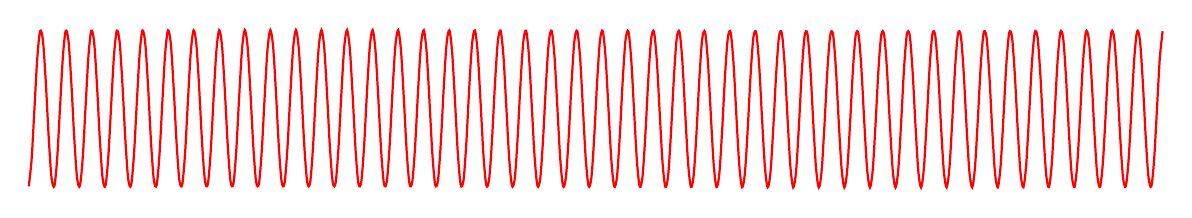
\begin{tikzpicture}[xscale=1.2]
    \draw[xscale=.3,thick,red,smooth,samples=400,domain=-20:20]
    plot({\x},{sin(400*\x)});
  \end{tikzpicture}
  
  {\footnotesize $\cos(400x)$}
  \caption{A wave with a well-defined wavelength}
  \label{fig:everywhere}
\end{figure}

In the figure, the particle (expressed as a wave) has a single wavelength
$\lambda$ (therefore a single value of momentum $p$, from
Eq.~\ref{eq:momentum-wavelength}), but it has no
distinguishing features that can tell you its location $x$. The bottom line is
that \textbf{when we have precise knowledge of a particle wave's momentum,
  then we have no knowledge of \emph{where} it is.} However, if a particle is
defined as waves with small variations of wavelengths, when we add up the
different waves together, we begin to see a \textbf{wave packet} emerge, as
shown in Fig.~\ref{fig:packet}.
\begin{figure}[ht]
  \centering
  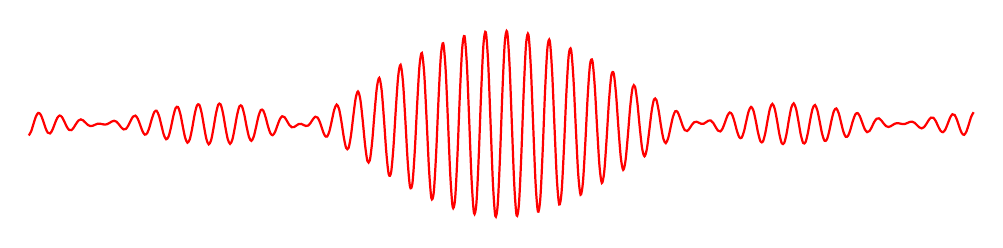
\begin{tikzpicture}
    \draw[xscale=.3,yscale=.07,thick,red,smooth,samples=400,domain=-20:20]
    plot({\x},{
      sin(400*\x)+
      sin(402.5*\x)+ sin(405*\x)+ sin(407.5*\x)+ sin(410*\x)+
      sin(412.5*\x)+ sin(415*\x)+ sin(417.5*\x)+ sin(420*\x)+
      sin(380*\x)+ sin(382.5*\x)+ sin(385*\x)+ sin(387.5*\x)+
      sin(390*\x)+ sin(392.5*\x)+ sin(395*\x)+ sin(397.5*\x)
    });
  \end{tikzpicture}
  
  {\footnotesize
    $\cos(380x)+\cos(382.5x)+\cdots+\cos(400x)+\cos(402.5x)+\cdots+\cos(420x)$
  }
  \caption{A wave with a spread of wavelengths}
  \label{fig:packet}
\end{figure}

\begin{wrapfigure}{r}{.2\textwidth}
  \centering
  \pic{.2}{Heisenberg.jpg}
  Werner Heisenberg
\end{wrapfigure}
The bottom line is that \textbf{in order to gain knowledge about the location
  of a particle, we \emph{must} give up information about its momentum.}
Because of the wave properties of particles, an observer can never be completely
certain of the relationship between an object's momentum $p$ and position $x$.
The more you know about an object's position, the less you know about its
momentum, and vice versa. The limitation, discovered by Werner
Heisenberg\footnote{1901--1976; Nobel prize winner in 1932} is called the
\textbf{Heisenberg uncertainty principle}:
\begin{equation}
  \boxed{\sigma_p\sigma_x\geq \frac{\hbar}{2}}
\end{equation}
%  \begin{center}
%    \begin{tabular}{l|c|c}
%      \rowcolor{pink}
%      \textbf{Quantity} & \textbf{Symbol} & \textbf{SI Unit} \\ \hline
%      Uncertainty in momentum  & $\sigma_p$ & \si{\kilo\gram.\metre/\second}\\
%      Uncertainty in position  & $\sigma_x$ & \si{\metre} \\
%      Redued Planck's constant & $\hbar$    & \si{\joule\second}
%    \end{tabular}
%  \end{center}
The quantity $\displaystyle\hbar=\frac{h}{2\pi}$ is called the
\textbf{reduced Planck's constant}.

\section{Atomic Model}
The ``orbital'' model of electrons does not work, because as the electron
orbits (accelerates around) the nucleus, it radiates electromagnetic radiation,
and therefore lose energy. The orbit will eventually collapse. A young Danish
physicist Niels Bohr postulated that electrons can move in certain
``non-radiating'' orbits, corresponding to energy levels:

It provides the first model that incorporates physicists' new knowledge of
quantum mechanics into the atomic model. Bohr began by assuming that a single
electron (with elementary charge $e$) is in a perfectly circular orbit around
a nucleus with $Z$ protons (with charge $Ze$, where $Z$ is called the
\textbf{atomic number}). The electrostatic force (coulomb force) therefore
provides the centripetal force keeping the electron in orbit:
\begin{equation}
  F_c=F_q=\frac{kZe^2}{r^2}
\end{equation}
From studying the motion of planets in circular orbits using gravity as the
centripetal force, the potential energy $U$, kinetic energy $K$ and total
energy $E$ for the atom in orbit can be expressed as:
\begin{equation}
  U=-\frac{kZe^2}{r}; \quad K=-\frac{kZe^2}{2r}=-\frac12 U;\quad
  \boxed{E=\frac{kZe^2}{2r}=\frac12 U}
\end{equation}
The total energy is one half of the potential energy, in agreement with the
study with gravity. (Thus far, the derivation is completely \emph{classical}.)
Bohr then applied the energy quantitation energy of Planck (Eq.~\ref{eq:nhf})

\begin{equation}
  \boxed{E_n=-\frac{k^2e^4m}{2\hbar^2}\frac{Z^2}{n^2}}
\end{equation}
  
From the wave-particle duality perspective, the ``orbits'' correspond more to
a standing wave around the nucleus (a standing wave does not lose energy)



%{Bohr Atomic Model}
%  \eq{-.1in}{
%    \boxed{E_n=-\frac{k^2e^4m}{2\hbar^2}\frac{Z^2}{n^2}}
%  }
%  \begin{center}
%    \begin{tabular}{l|c|c}
%      \rowcolor{pink}
%      \textbf{Quantity} & \textbf{Symbol} & \textbf{SI Unit} \\ \hline
%      Energy at level $n$ & $E_n$ & \si{\joule} \\
%      Coulomb's constant & $k$ & \si{N.m^2/C^2} \\
%      Elementary charge  & $e$ & \si{\coulomb} \\
%      Atomic mass        & $m$ & \si{\kilo\gram} \\
%      Reduced Planck's constant & $\hbar$ & \si{\joule.\second}\\
%      Atomic number      & $Z$ & integer; no units\\
%      Energy level       & $n$ & integer; no units
%    \end{tabular}
%  \end{center}
%
%
%
%{Bohr Atomic  Model}
Successful in describing the behaviour of the hydrogen atom---but fails for
heavier atoms---although it still relies on 
\begin{itemize}[noitemsep,topsep=0pt]
\item Quantization of energy (new physics!)
\end{itemize}
De Broglie's hypothesis gives us a glimpse of what Bohr is missing
\begin{itemize}[noitemsep,topsep=0pt]
\item The ``orbits'' correspond to a standing wave around the nucleus
\item A standing wave does not lose energy
\end{itemize}

\section{Hydrogen Emission}
%  
%
%    \column{.6\textwidth}
%    \begin{itemize}
%    \item Lyman series:
%      \begin{itemize}
%      \item the EM emissions when the electrons drop from a higher energy state
%        ($E_n$) to the ground state $n=1$ (i.e.\ $E_1$)
%      \item The frequency is given by:
%        
%        \eq{-.2in}{
%          f=\frac{E_1-E_n}{h}
%        }
%      \item We can apply universal wave equation to get the wavelengths
%      \end{itemize}
%    \item Balmer series--dropping to $E_2$
%    \item Paschen series--dropping to $E_3$
%    \end{itemize}
%
%    \column{.4\textwidth}
%    \pic{1}{400px-Hydrogen_transitions.png}
%  
%
%
%
%
%  \frametitle{Standing Wave on a String}
%  
%    \column{.3\textwidth}
%    \pic{1}{strhar.png}
%
%    \column{.7\textwidth}
%    \begin{itemize}
%    \item We have studied standing waves in Grade 11
%    \item If electron is to be in a ``stable orbit'' around a nucleus, it has
%      to be in a standing wave pattern
%    \item Otherwise, it will interfere with itself
%    \end{itemize}
%  
%
%
%
%
%  \frametitle{Circular Standing Wave}
%  \begin{center}
%    \pic{.7}{oo1wp.png}
%  \end{center}
%  Electron resonance states $n=3,4,5,6$
%
\section{Schrodinger Equation}


\subsection{Particle in a Box}

\begin{wrapfigure}{l}{.3\textwidth}
  \pic{.3}{../box.png}
  \caption{Energy states of the particle in a box.}
  \label{fig:1d-box}
\end{wrapfigure}
A particle in a 1D box has to behave like a standing wave. The resonance modes
(frequencies where a stable standing wave exists) correspond to the wavelengths:
\begin{equation}
  \lambda=\frac{2L}{n}\quad n=1,2,3\ldots
\end{equation}
and the momentum of the particle is:
\begin{equation}
  p=\frac{h}{\lambda}=\frac{nh}{2L}
\end{equation}
%  
%
%
%
%
%{Particle in a Box}
%  
%    \column{.3\textwidth}
%    \pic{1}{box.png}
%    
%    \column{.7\textwidth}
The kinetic energy $K$ of the particle can be expressed in terms of momentum
$p$:
\begin{equation}
  K_n=\frac{1}{2}mv^2=\frac{p^2}{2m}=\frac{n^2h^2}{8mL^2}
\end{equation}
If a particle is a standing wave, then kinetic energy of the particle can never
be zero (as long as it is confined inside the box), therefore
\begin{itemize}[noitemsep,topsep=0pt]
\item It cannot have zero velocity
\item The lowest energy level ($n=1$) is called the \textbf{zero-point energy}
\end{itemize}
%  
%
%
%
%
%  \frametitle{Example}
%  \textbf{Example 3:} A \SI{.150}{\kilo\gram} billiard ball is confined to the
%  pool table \SI{1.42}{\metre} wide. How long (in seconds) will it take to
%  travel from one side of the table to the other? (Use fundamental mode.)
%
%
\end{document}
